\documentclass[12pt]{article}
\usepackage[utf8]{inputenc}
\usepackage{parskip}
\usepackage[a4paper, margin=1.5in]{geometry}
\usepackage{graphicx}
\usepackage{hyperref}
\usepackage{listings}
\usepackage{array}
\usepackage{minted}
\usepackage{enumitem}

\renewcommand{\arraystretch}{1.5}

\title{Project Report - Control tower}
\date{\today}
\author{Federico Fregosi}

\begin{document}
\pagenumbering{gobble}
\maketitle
\vfill

\tableofcontents
\vfill
\clearpage
\setcounter{page}{1}
\pagenumbering{arabic}

\section{Introduction}
\subsection{Overview}
Consider a system that simulate an airport. The airport is composed by one runway, one parking area and one control tower. The runway is used for landing/take-off and can be occupied by only one plane at a time, whereas the parking area can contain one or more of them simultaneously. The control tower manages the air traffic of the airport by making the runway available for planes that needs. When the runway is occupied, planes that need it for landing or take-off are placed respectively in the landing queue or in the take-off queue. When the runway is unoccupied instead, the control tower serves one airplane in a queue according to the policy that take-off has priority over landing. Every plane has a specific set of values:
\begin{itemize}
	\item t\textsubscript{l} = time necessary to perform the landing operation
	\item t\textsubscript{p} = time that the airplane will spend in the parking area
	\item t\textsubscript{o} = time necessary to perform the take-off operation
\end{itemize}
After landing, a plane go in the parking area whereas after a plane take-off, it leaves the system.

\subsection{Objectives}
In this analysis, the following objectives will be investigated:
\begin{itemize}
	\item relationship between the service times and the waiting time in both landing and take-off queues;
	\item optimal value for the size of the parking area in order to be sure of having space but also to not waste too much space.
\end{itemize}

\subsection{Performance indexes}
In order to fulfill the above-stated objectives, the following performance indexes will be taken into consideration:
\begin{itemize}
	\item
	\item 
\end{itemize}

\subsection{Scenarios}
The following scenarios will be taken into consideration:
\begin{itemize}
	\item constant interarrivals times, constant service times (only for code verification since in this scenario no queuing is possible and thus it is of no interest);
	\item exponential distribution of interarrivals times, exponential distribution of service times;
\end{itemize}
where interarrivals times are the times at which a plane ask for landing, whereas service times are t\textsubscript{l}, t\textsubscript{p}, t\textsubscript{o}.


\section{Model}
\subsection{Description}

\subsection{Assumption}
The following assumption were made when modeling the system:
\begin{itemize}
	\item both landing and take-off queue have infinite queuing space;
	\item the parking area has infinite capacity;
	\item planes cannot leave the queues;
	\item planes cannot change their position in queue;
	\item all the service times of a planes are independent RVs.
\end{itemize}

\section{Implementation}
\subsection{Code Overview}
The model is composed by three nodes:
\begin{itemize}
	\item \textbf{Airspace}: the node in which planes are created and initialized before reaching the control tower asking for a landing operation
	\item  \textbf{Control tower}: the main node of the system. It is responsible for the manage of both landing and take-off queues and operations
	\item  \textbf{Parking area}: node in which planes spend the t\textsubscript{p} time
\end{itemize}
Note that the runway isn't a node itself, but it is included into the control tower.
Each plane has to follow all the following steps before leaving the system:

\begin{figure}[h!]
    \centering
    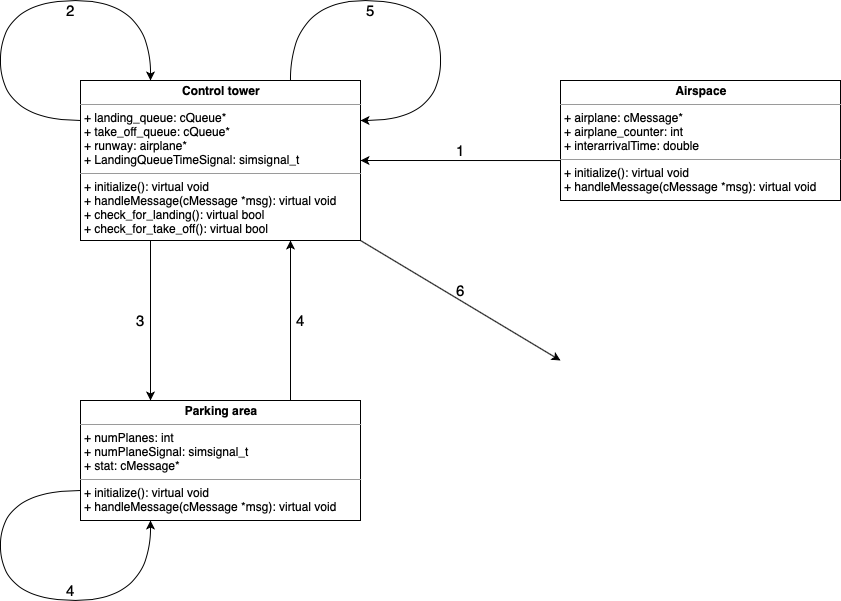
\includegraphics[scale=0.45]{immagini/lifecycle}
    \caption{Life-cycle of each airplane}
    \label{fig:life-cycle of each airplane}
\end{figure}

\begin{enumerate}[label=\arabic*)]
	\item the airplane queues for landing;
	\item the airplane perform the landing operation, which takes a time t\textsubscript{l};
	\item the airplane go in the parking area and remains there for t\textsubscript{p};
	\item the airplane queue for take-off;
	\item the airplane performs the take-off operation, which takes a time t\textsubscript{o};
	\item the airplane leaves the system.
\end{enumerate}

\end{document}